
%\flushright{\hyperref[index]{\color{black!65}{Ritorna all'indice}}}\flushleft

	\section{A} \label{sec:A} 
		
		\subsection{AMMINISTRATORE} \index{Amministratore} \label{amministratore}
		È uno dei \underline{\hyperref[ruoli]{ruoli}} in un progetto. Controlla l'ambiente di lavoro. Si occupa di amministrare le infrastrutture di supporto, risolvere problemi legati alla gestione dei processi, gestire la documentazione di progetto e controllare \underline{\hyperref[versione]{versioni}} e \underline{\hyperref[configurazione]{configurazioni}}.
		
		\subsection{ANALISI DEI REQUISITI} \index{Analisi dei requisiti} \label{analisideirequisiti} %V.I
		L' Analisi dei \underline{\hyperref[requirements]{requisiti}} è lo step dopo lo Studio di fattibilità e tratta sostanzialmente di capire appieno il problema. Riguarda la \underline{\hyperref[qualifica]{qualifica}} e se ne occupa l'\underline{\hyperref[analista]{Analista}} che deve cercare di entrare nell'ottica dell'utente. Lo svolgimento dell'analisi prevede lo studio dei bisogni e delle fonti del dominio applicativo, una prima classificazione dei requisiti, una modellazione concettuale del sistema, l'assegnazione dei requisiti alle varie parti del sistema e la negoziazione con il committente. Dopodiché avviene la redazione del \underline{\hyperref[piano]{Piano}} di qualifica per metodi, tecniche, strumenti, tempi ecc. \\
		
		Le \textit{attività} di analisi sono:
			\begin{itemize}
				\item studiare e definire il problema da risolvere, identificando il prodotto da commissionare (compito del cliente), capendo cosa deve essere realizzato e definendo gli accordi contrattuali;
				\item verificare il costo e la \underline{\hyperref[qualita]{qualità}} in base ai \underline{\hyperref[requirements]{requisiti}} derivanti dal cliente;
				\item (lato fornitore) studio dei bisogni e delle fonti, identificando, specificando e classificando i \underline{\hyperref[requirements]{requisiti}};
				\item (lato fornitore) modellazione concettuale del sistema con partizionamento in componenti (ambiti) a scopo di	allocazione dei requisiti (per esempio con diagrammi d'uso);
				\item (lato fornitore) ripartizione dei requisiti a parti del sistema;
				\item accertare la soddisfacibilità dei requisiti rispetto ai
				vincoli di processo;
				\item assicurare, tramite \underline{\hyperref[tracciamento]{tracciamento}}, che i requisiti concordati siano tutti e soli quelli necessari (tutti i requisiti in AR	soddisfano un particolare bisogno) e sufficienti (tutti i bisogni rilevati nelle fonti sono requisiti in AR);
				\item determinare con il cliente l’utilità strategica dei
				\underline{\hyperref[requirements]{requisiti}} concordati;
				\item adozione di norme redazionali (aiuta a evitare espressioni ambigue) e glossario (aiuta a garantire terminologia consistente);
				\item uso di metodi (semi-)formali (aiuta a ridurre
				gli errori di interpretazione) come diagrammi e formule;
			\end{itemize}
		
		I \textit{processi di supporto} implicati da esse sono:
			\begin{itemize}
				\item documentazione, al fine di raccogliere i risultati dello studio di fattibilità e specificare i requisiti;
				\item gestione e \underline{\hyperref[manutenzione]{manutenzione}} dei prodotti, comprendente il \underline{\hyperref[tracciamento]{tracciamento}} dei requisiti, impostazione e gestione della configurazione e dei cambiamenti;
			\end{itemize}
		
		All'interno del nostro progetto possiamo quindi dire di avere diversi prodotti documentali: per \textit{definire} i bisogni (utente e SW) abbiamo il \underline{\hyperref[capitolati]{capitolato d'appalto}}, per \textit{specificare} abbiamo appunto l'Analisi dei Requisiti (che è un documento contrattuale) e lo \underline{\hyperref[studiofattibilita]{Studio di Fattibilità}} (che è un documento interno del fornitore). Per la \textit{ripartizione} dei requisiti invece la questione è molto delicata perchè da qui inizia la \underline{\hyperref[progettazione]{Progettazione}}. Il confine tra Analisi e Progettazione è molto sottile: per esempio, l'\underline{\hyperref[analista]{Analista}} riesce già a vedere dei sotto-problemi che poi però sono compito di chi progetta. 
		
		\begin{figure}[H]
			\centering
			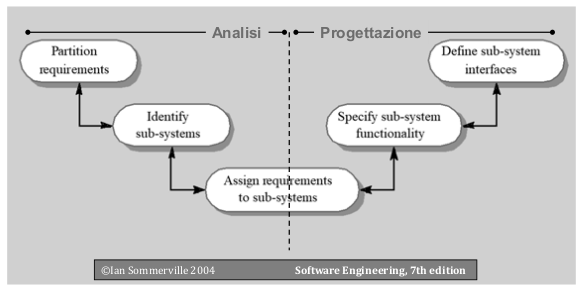
\includegraphics[width=0.8\textwidth]{img/conf}		
			\caption{Confine tra Analisi e Progettazione.}
		\end{figure} 
		
		Ci sono diversi approcci su come procedere per l'Analisi dei Requisiti:
			\begin{itemize}
				\item \textbf{\underline{\hyperref[topdown]{Top-down}}}
				\item \textbf{\underline{\hyperref[bottomup]{Bottom-up}}}
				\item \textbf{Agile} \label{agile}
				Generalmente parto da un'idea di una cosa che già esiste e penso alle funzionalità da poterci aggiungere. É una via di mezzo tra le altre due.
			\end{itemize}	
		
		Le \textit{tecniche} di analisi comprendono:
			\begin{itemize}
				\item l'interazione con il cliente (il cui esito viene documentato), tramite interviste o discussione di scenari;
				\item discussioni creative e collaborative, ovvero \underline{\hyperref[brainstorming]{brainstorming}};
				\item prototipazione,interna (per il fornitore) o esterna (per la discussione con il cliente);
				\item la comprensione del dominio, che prevede: una serie di domande base come \textit{A quali bisogni risponde il prodotto atteso?} e \textit{Quali problematiche d’uso esso comporta}, l'acquisizione delle conoscenze tramite documentazione preesistente e interviste ai potenziali utenti, consolidamento del glossario che raccoglie e definisce i termini chiave del dominio per avere un'interazione ordinata con il committente;
			\end{itemize}
		
		Capita a volte che il progetto venga abbandonato e le principali cause sono:
			\begin{itemize}
				\item \underline{\hyperref[requirements]{requisiti}} incompleti;
				\item insufficiente coinvolgimento del cliente e/o dell’utente (non sono necessariamente la stessa entità);
				\item scarsità di risorse;
				\item attese irrealistiche;
				\item nsufficiente competenza tecnologica e/o metodologica del fornitore;
			\end{itemize}
		
		Mentre gli stati di progresso secondo \underline{\hyperref[semat]{SEMAT}} sono
			\begin{itemize}
				\item \textit{Conceived}: il \underline{\hyperref[committente]{committente}} è identificato e gli \underline{\hyperref[stakeholder]{stakeholder}} vedono sufficienti opportunità per il progetto;
				\item \textit{Bounded}: bisogni macro sono chiari e i meccanismi di \underline{\hyperref[gestionerequisiti]{Gestione dei requisiti}} (\underline{\hyperref[configurazione]{configurazione}} e cambiamento) sono fissati;
				\item \textit{Coherent}: i requisiti sono classificati e quelli essenziali (obbligatori) sono chiari e ben definiti;
				\item \textit{Acceptable}: i requisiti fissati definiscono un sistema soddisfacente per gli stakeholder;
				\item \textit{Addressed}: il prodotto è pronto al rilascio e all'uso;
				\item \textit{Fulfilled}: il prodotto merita la piena approvazione degli stakeholder tanto soddisfa i requisiti;
			\end{itemize}
		
		
		%\subsection{ANALISI DEI RISCHI} \index{Analisi dei rischi} \label{analisirischi} %?
		
		\subsection{ANALISTA} \index{Analista} \label{analista}
		È uno dei \underline{\hyperref[ruoli]{ruoli}} in un progetto. Generalmente sono pochi ma hanno molta influenza sul successo del progetto. Conosce il dominio del problema e ha esperienza professionale, ma raramente segue il progetto fino alla consegna.
		
		\subsection{APPROCCIO} \label{approccio} \index{Approccio}
		Avvicinarsi/predisporsi. Può essere:
			\subsubsection{Sistematico} \label{sistematico}
			ovvero lavorando in maniera metodica (ho un metodo da seguire che mi precede) e rigorosa usando ed evolvendo la \underline{\hyperref[best]{best practice}} [importante il tempo];
			\subsubsection{Disciplinato} \label{disciplinato}
			ovvero seguendo regole fissate. Per essere disciplinato ho bisogno di due documenti: Norme per fissare il metodo, Piano di Progetto per il quando faccio.
			\subsubsection{Quantificabile} \label{quantificabile}
			ovvero che permette di misurare \underline{\hyperref[efficienza]{efficienza}} ed \underline{\hyperref[efficacia]{efficacia}}. Il nostro fare deve produrre cose buone \textbf{oggettivamente}. Ci interessa misurare la qualità, per vedere il raggiungimento degli obiettivi che mi sono data.
			
		\subsection{ARCHITECTURE SELECTED}	\index{Architecture Selected}	\label{architectureselected}
		L'architettura viene capita e selezionata, oltre alla selezione delle tecnologie necessarie.	
			
		\subsection{ARCHITETTURA}	\index{Architettura} \label{architettura}
		Si intende architettura logica: è di alto livello (quindi non implementato, concettuale) e consiste nel dividere in parti per massimizzare il parallelismo. Si divide fino a che non se ne trae più vantaggio (fino a che il costo della divisione diventa più un onere che un beneficio).
		Riporta UNA soluzione che soddisfa il cliente.
		L'architettura:
		\begin{itemize}
			\item Decomposta (suggerisce l'idea di top-down) in \underline{\hyperref[componente]{componenti}}.
			\item Ha un'organizzazione: le componenti stanno insieme secondo regole date e ognuna ha un ruolo preciso e collabora.
			\item Definisce le interfacce: qual è il modo in cui le componenti collaborano (parola associata a protocollo (=accordo) perché un'interfaccia si appoggia a un protocollo).
			\item Paradigmi (=come si fa) di composizione: componenti messe insieme secondo regole, limiti, vincoli. Definisce come vengono organizzate.
		\end{itemize}
		Le architetture hanno scelte di paradigmi ed esistono più stili architetturali che determinano l'organizzazione dell'informazione di stato e l'interazione tra le parti
		\underline{\hyperref[qualita]{Qualità}} di una buona architettura: %slide 11/36
		\begin{itemize}
			\item \textbf{Modularità}: (legata a Incapsulazione e Disponibilità) ha l'obiettivo di minimizzare la dipendenza tra parti. Ha due opzioni
			\begin{enumerate}
				\item Suddivide come la pipeline è divisa in stadi;
				\item In modo resiliente, ovvero facendo \textit{information hiding} altrimenti si espone ciò che è "implementation detail" (deve essere ben nascosto perchè altrimenti confonde e dà disagio);
			\end{enumerate}
			\item \textbf{Sufficienza}: deve soddisfare tutti i requisiti, coprire il bisogno;
			\item \textbf{Comprensibilità}: deve essere capita dagli stakeholder, anche perché ci sono diversi stili;
			\item \textbf{Robustezza}: sta in piedi anche se cambio un modulo;
			\item \textbf{Flessibilità}: non deve collassare, deve essere in grado di evolvere (attuando modifiche a costo contenuto);
			\item \textbf{\underline{\hyperref[riuso]{Riusabilità}}}: fare nell'intento che possa essere buono anche per altri in futuro;
			\item \textbf{Efficienza}: senza eccesso di risorse;
			\item \textbf{Affidabilità}: quando c'è bisogno di utilizzarla, fa le cose che deve;
			\item \textbf{Disponibilità}: stare in piedi senza grande bisogno di manutenzione (se una parte è sotto manutenzione, non deve essere interrotto tutto il sistema);
			\item \textbf{Sicurezza rispetto a malfunzionaamenti}: \textit{"safety"}, non ho malfunzionamenti che fanno danno;
			\item \textbf{Sicurezza rispetto a intrusioni}: \textit{"security"}, invulnerabile rispetto alle intrusioni. Mitigare il rischio e massimizzare i vantaggi;
			\item \textbf{Semplicità}: le parti contengono solo il necessario, niente di superfluo;
			\item \textbf{Incapsulazione}: (\textit{Information hiding}) l'interno delle componenti non è visibile dall'esterno, quindi i clienti conoscono solo l'interfaccia, aumenta la manutenibilità e la possibilità di \underline{\hyperref[riuso]{riuso}};
			\item \textbf{\underline{\hyperref[coeso]{Coesione}}}: le parti che stanno insieme hanno gli stessi obiettivi e ognuna ha un ruolo (la coesione si può misurare);
			\item \textbf{Basso accoppiamento}: (l'accoppiamento è la nemesi della coesione, quando viene mossa una parte ne viene conseguentemente mossa anche un'altra) distinte parti che dipendono poco o niente le une dalle altre, ma quando dall'esterno fanno assunzioni su come certe cose stiano all'interno di altre e quando si condividono frammenti delle stesse risorse (bisogna cercare di massimizzare l'indice di utilità e minimizzare l'indice di dipendenza);
		\end{itemize}
		L'architettura definisce i {\underline{\hyperref[ruoli]{ruoli}}}.	
		Tutte le qualità delle caratteristiche attese vanno perseguite. %slide 2/30 verifica e validazione
		Tutto va sottoposto a verifica.
	
		\subsection{AUDIT PROCESS} \index{Audit Process} \label{audit}
		Imporre un andamento e assicurarsi che l'attività che si sta facendo si svolga nel migliore dei modi possibili. Permette di migliorare il \underline{\hyperref[way]{way of working}}. È una revisione \textbf{esterna}.
		
	
